\chapter{拓扑空间}

\section{拓扑空间}

由于拓扑变化不允许将图形撕裂，因此拓扑变换实际上是一系列的连续变换，因此先回忆一下之前除了使用$\varepsilon-\delta$语言外的另一种连续函数的刻画方法.

\begin{theorem}{}
    $f:\mathbb{R}\to\mathbb{R}$是连续函数当且仅当任何开集的原像是开集.
\end{theorem}

关于开集，它有以下的性质.

\begin{proposition}{实数集上开集的性质}
    \begin{enumerate}
        \item $\varnothing$和$\mathbb{R}$是开集.
        \item 任意多个开集的并还是开集.
        \item 任意有限多个开集的交还是开集.
    \end{enumerate}
\end{proposition}
\begin{proof}
    第三条性质的证明：设$U_1=\bigcup_\alpha{(a_\alpha,b_\alpha)},U_2=\bigcup_\beta{(c_\beta,d_\beta)}$.\par
    则$U_1\cap U_2=\left(\bigcup_\alpha{(a_\alpha,b_\alpha)}\right)\cap\left(\bigcup_\beta{(c_\beta,d_\beta)}\right) = \bigcup_{\alpha,\beta}\big((a_\alpha,b_\alpha)\cap(c_\beta,d_\beta)\big)$.\par
    其中$(a_\alpha,b_\alpha)\cap(c_\beta,d_\beta)$一定是空集或是开区间，所以$U_1\cup U_2$也是开集.\par
    对于有限多个的情形应用数学归纳法即可.\par
\end{proof}

常规意义上$\mathbb{R}$上的开集都是$\mathbb{R}$的子集，因此它们构成了$\mathbb{R}$的一个子集族.如果将开集所满足的三个性质抽象出来，考察$\mathbb{R}$的任意子集族是否满足这三条性质，就得到了\bluebf{拓扑空间}的概念.

\begin{definition}{拓扑空间}
    设$X$是一个集合，$\mathcal{T}$为$X$上的子集族，满足：
    \begin{enumerate}
        \item $\varnothing,X\in\mathcal{T}$
        \item $\mathcal{T}$中任意子集的并仍属于$\mathcal{T}$
        \item $\mathcal{T}$中有限个子集的交仍属于$\mathcal{T}$
    \end{enumerate}
    则称$\mathcal{T}$为$X$上的\textbf{拓扑}，$(X,\mathcal{T})$为一个\textbf{拓扑空间}，$\mathcal{T}$中的子集称为\textbf{开集}.
\end{definition}

应用数学归纳法，其中的条件3还可以予以弱化.
\begin{proposition}{条件3的等价条件}
    $\mathcal{T}$中有限个子集的交仍属于$\mathcal{T} \Leftrightarrow \mathcal{T}$中两个子集的交属于$\mathcal{T}$.
\end{proposition}

\begin{instance}
    (1)在标准的实数集$\mathbb{R}$中，$\mathcal{T}:=\left\{\bigcup_\lambda{(a_\lambda,b_\lambda)}\left|(a_\lambda,b_\lambda)\text{是}\mathbb{R}\text{上的开区间}\right.\right\}$是拓扑空间.\par
    (2)$X=\{a,b,c\}$，$\mathcal{T}_1 = \left\{\varnothing,X,\{a\},\{b\},\{a,b\}\right\}$，$\mathcal{T}_2 = \left\{\varnothing,X,\{a\},\{a,b\}\right\}$，$\mathcal{T}_3 = \left\{\varnothing,X,\{a\},\{a,c\}\right\}$.\par
    但$\left\{\varnothing,X,\{b\},\{c\},\{a,b\}\right\}$不是拓扑，因为$\{b\}\cup\{c\}=\{b,c\}$不在其中.\par
    (3)$X$是一个非空集合，$\mathcal{T}_1=\{\varnothing,X\}$，被称为\bluebf{平凡拓扑}.$\mathcal{T}_2=2^X$，被称为\bluebf{离散拓扑}.\par
    (4)$X=\mathbb{R},\mathcal{T}=\{\varnothing\cup\{\mathbb{R}\text{上有限子集的补集}\}\}$.
    \begin{enumerate}[leftmargin=4.75em,label=(\roman*)]
        \item $\varnothing,\mathbb{R} \in \mathcal{T}$
        \item $\bigcup_{\lambda}{\left(\mathbb{R}\setminus F_\lambda\right)}=\mathbb{R}\setminus\left(\bigcap_{\lambda}{F_\lambda}\right) \in \mathcal{T}$
        \item $(\mathbb{R}\setminus F_1) \cap (\mathbb{R}\setminus F_2)=\mathbb{R}\setminus\left(F_1\cup F_2\right) \in \mathcal{T}$
    \end{enumerate}
    因此$\mathcal{T}$是$\mathbb{R}$上的拓扑，称为\bluebf{有限补拓扑}，记作$\mathbb{R}_{fc}$.
\end{instance}

由上面的例子可以看出，在同一个集合上可以定义不同的拓扑(至少有平凡拓扑和离散拓扑两种拓扑)，不同的拓扑之间可以用以下关系比较.

\begin{definition}{拓扑的精细与粗糙}
    设$\mcal{T}_1,\mcal{T}_2$是集合$X$上的两个拓扑，如果$\mcal{T}_1\subset \mcal{T}_2$，则称$\mcal{T}_2$比$\mcal{T}_1$\textbf{精细}，或称$\mcal{T}_1$比$\mcal{T}_2$\textbf{粗糙}.
\end{definition}
特别地，如果定义中的包含加强为真包含，称\bluebf{严格精细}和\bluebf{严格粗糙}.
\begin{conclusion}
    平凡拓扑是最粗糙的拓扑，因为它仅包含了空集和全集，是满足条件1的最低要求.\par
    离散拓扑是最精细的拓扑，因为它已经包含了集合中的所有子集.\par
\end{conclusion}

\begin{instance}
    在$\mathbb{R}$上，$\mathbb{R}_{trivial}\subsetneqq\mathbb{R}_{fc}\subsetneqq\mathbb{R}_{std}\subsetneqq\mathbb{R}_{discrete}$.\par
    其中$\mathbb{R}_{fc}\subsetneqq\mathbb{R}_{std}$的原因在于任意有限集的补集都是$\mathbb{R}_{std}$中的开集，因此$\mathbb{R}_{fc}\subset \mathbb{R}_{std}$.并且如果我们取$\mathbb{R}_{std}$中的开集$(0,1)$，它的补集是一个无限集，因此不在$\mathbb{R}_{fc}$中，所以$\mathbb{R}_{fc}\subsetneqq \mathbb{R}_{std}$是严格包含的关系.
\end{instance}

但并非所有的拓扑都可以比较大小，如下例所示：
\begin{instance}
    $X=\{a,b,c\},\mcal{T}_1=\{\varnothing,X,\{a\},\{a,b\}\},\mcal{T}_2=\{\varnothing,X,\{a\},\{a,c\}\}$，这两个拓扑无法比较大小.
\end{instance}


\begin{definition}{邻域}
    设$X$是一个拓扑空间，$x\in X$，任意包含$x$的\uline{开集}$U$称为$x$的一个\textbf{邻域}.
\end{definition}

\begin{theorem}{}
    设$A\subset X$，则$A$是开集当且仅当$\forall\, x\in A,\exists\, x\,\text{的一个邻域}\,U,\st x\in U\subset A$.
\end{theorem}\par
\begin{proof}
    “$\Rightarrow$” 显然成立.\par
    \begin{wrapfigure}{r}{0.12\textwidth}
    \vspace{-3 em}
    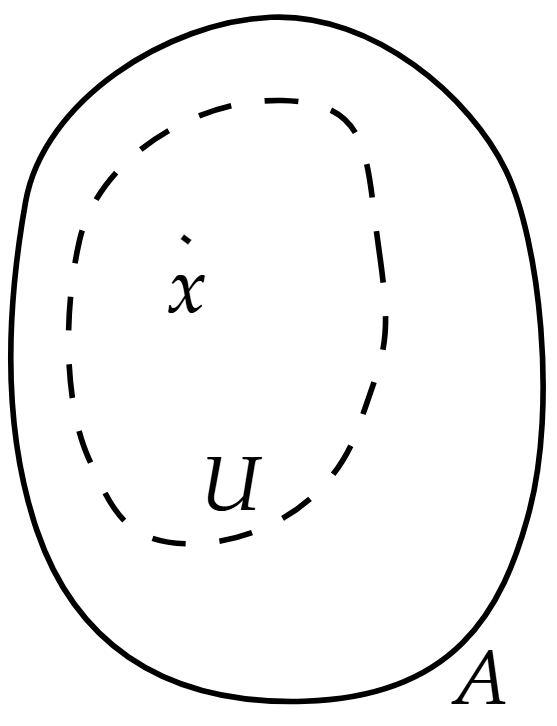
\includegraphics[width=0.12\textwidth]{fig/2.1.1.png}
    \vspace{0 em}
    \end{wrapfigure}
    “$\Leftarrow$” $\forall\, x \in A,\exists\, x\text{的一个邻域}\,U_x,\st x\in U_x\subset A$，所以$A=\bigcup_{x\in A}{U_x}$.\par
    由于$U_x$是$X$的一个开集，所以$A$是一个开集.    
\end{proof}

\section{拓扑基}
\vspace{-1 em}
\begin{definition}{拓扑基}
    设$X$是一个集合，$\mcal{B}$是$X$的子集族，若$\mcal{B}$满足条件：
    \begin{enumerate}
        \item $\forall\, x\in X,\exists\, B\in\mcal{B},\st x\in B,\ie X=\bigcup_{B\in\mcal{B}}{B}$
        \item 若$B_1,B_2\in\mcal{B},x\in B_1\cap B_2$，则$\exists\, B\in\mcal{B},\st x\in B\subset B_1\cap B_2$
    \end{enumerate}
    则称$\mcal{B}$为$X$的\textbf{拓扑基}.
\end{definition}
下图直观地展示了拓扑基的第二个条件.
\begin{figure}[h]
    \centering
    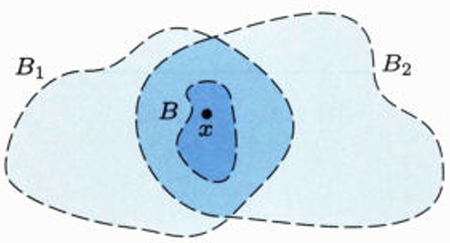
\includegraphics[width=0.5\textwidth]{fig/2.2.1.png}
    \captionof{figure}{拓扑基的特性}
\end{figure}

\begin{theorem}{拓扑基生成拓扑}
    设$\mcal{B}$为$X$的拓扑基，$\mcal{T}=\{\mcal{B}\text{中任意多个子集的并}\}$，则$\mcal{T}$是$X$上的拓扑，称其为由拓扑基$\mcal{B}$生成的拓扑，$\mcal{B}$中的子集称为\textbf{基元素}.
\end{theorem}

\begin{proof}
    \begin{enumerate}[label=(\roman*)]
        \item $\varnothing,X\in\mcal{T}$
        \item 对任意并的封闭性显然
        \item $U_1=\bigcup_{\alpha}{B_\alpha},U_2=\bigcup_{\beta}{C_\beta},\; B_\alpha,C_\beta\in\mcal{B}$，则$U_1\cap U_2=\bigcup_{\alpha,\beta}({B_\alpha\cap C_\beta})\in\mcal{T}$.\par
        由条件2，$\forall\, x\in B_\alpha\cap C_\beta,\exists\, D_x\in \mcal{B},\st x\in D_x\subset B_\alpha\cap C_\beta$.\par
        因此$B_\alpha\cap C_\beta = \bigcup_{x\in B_\alpha\cap C_\beta}{D_x} \xLongrightarrow{D_x\in\mcal{T}} B_\alpha\cap C_\beta\in\mcal{T}$.\par
        所以$U_1\cap U_2\in\mcal{T}$.\par
    \end{enumerate}
\end{proof}


\begin{instance}
    在$\mathbb{R}_{std}$上，$\mcal{B}=\{\mathbb{R}\text{中所有开区间}\}$，$\mcal{B}$生成$\mathbb{R}_{std}$.
\end{instance}

\begin{instance}
    $X\neq\varnothing,\mcal{B}=\{\{x\}|x\in X\}$，$\mcal{B}$生成$X$上离散拓扑.
\end{instance}

上述的$\mcal{B}$一定是一个拓扑基，条件1显然，而$\mcal{B}$中的所有元素都是单点集，因此交集为空，自然条件2成立.

\begin{instance}
    在$\mathbb{R}$上，$\mcal{B}=\{\left[a,b\right)|a<b\}$是一个拓扑基，验证其确为一个拓扑基.\par
    \begin{enumerate}[leftmargin=3.75em]
        \item $\forall\, x\in\mathbb{R},x\in[x,x+1)\in \mcal{B}$
        \item $[a,b)\cap[c,d) = [\max\{a,c\},\min\{c,d\})$.\par
        则$\forall\, x\in [a,b)\cap[c,d),x\in[\max\{a,c\},\min\{c,d\})$
    \end{enumerate}\par
    $\mcal{B}$生成了$\mathbb{R}$上的拓扑，称为\bluebf{下极限拓扑}，记作$\mathbb{R}_l$.
\end{instance}


\begin{lemma}{拓扑基的充分条件}\label{lem:2.1}
    假设$\mcal{B}$是$X$中的子集族，如果$\mcal{B}$满足：
    \begin{enumerate}
        \item $\forall\, x\in X,\exists\, B\in\mcal{B},\st x\in B$.
        \item $B_1,B_2\in\mcal{B}\Rightarrow B_1\cap B_2=\varnothing\,\text{或}\,B_1\cap B_2\in\mcal{B}$
    \end{enumerate}
    则$\mcal{B}$是$X$的拓扑基.
\end{lemma}
从上述引理中可以看出，相较于$X$上的拓扑，$X$上的拓扑基所满足的条件更加简单，它是更加规则的集合.

\begin{lemma}{开集的描述}\label{lem:2.2}
    设$X$是一个集合，$\mcal{B}$是$X$上一个拓扑基，则$U\subset X$在由$\mcal{B}$生成的拓扑中是开集当且仅当$\forall\, x\in U,\exists\, B_x\in\mcal{B},\st x\in B_x\subset U$.
\end{lemma}
\begin{proof}
    “$\Rightarrow$” 根据定义，存在一组基元素$B_\lambda,\lambda\in\Lambda$，使得$U=\bigcup_{\lambda\in\Lambda}{B_\lambda}$.\par
    $\forall\, x\in U,x\in\bigcup_{\lambda\in\Lambda}{B_\lambda}\Rightarrow\exists\, \lambda \in \Lambda, \st x\in B_\lambda\subset U$.取$B_x=B_\lambda$即可.\par
    “$\Leftarrow$” 根据假设，$U=\bigcup_{x\in U}{B_x}$，$U$是一组基元素的并.因此$U$是开的.
\end{proof}

下面举几个拓扑基及其生成的拓扑的例子.
\begin{instance}
    考虑$\mathbb{R}$，$\mcal{B}=\{(a,b),(a,b)-K\}$，其中$K=\left\{\frac{1}{n}\Big|n\in\mathbb{Z}^+\right\}$，
    则$\mcal{B}$是拓扑基.\par
    $(a,b)\cap \left((c,d)-K\right)=(\max\{a,c\},\min\{b,d\})-K$.\par
    $\left((a,b)-K\right)\cap \left((c,d)-K\right)=(\max\{a,c\},\min\{b,d\})-K$.\par
    因此$\mcal{B}$是$\mathbb{R}$上的一个拓扑基，它生成的拓扑称为\bluebf{K-拓扑}.\par
\end{instance}

\begin{instance}
    考虑$\mathbb{R}$，$\mcal{B}=\big\{\left[n,n+1\right)|n\in\mathbb{Z}\big\}$是拓扑基.\par
    其原因为，任意两个这样的左闭右开区间，如果它们两个相同，则交集就是自身，否则交集为空.
\end{instance}


考虑$X=\mathbb{R}^n$，若$x=(x_1,x_2,\cdots,x_n),y=(y_1,y_2,\cdots,y_n)\in\mathbb{R}^n$，定义两点距离为欧氏距离，即$d(x,y)=\sqrt{(x_1-y_1)^2+\cdots+(x_n-y_n)^2}$.定义其中的开球为$B(x,\varepsilon)=\left\{y\in\mathbb{R}^n|d(x,y)<\varepsilon\right\}$.把所有开球的集合记为$\mcal{B}_1=\left\{B(x,\varepsilon)\subset\mathbb{R}^n|x\in\mathbb{R}^n,\varepsilon>0\right\}$.那么我们就有以下的引理\par
\begin{lemma*}
        $\mcal{B}_1$是$\mathbb{R}^n$上的拓扑基.
\end{lemma*}
    \begin{wrapfigure}{r}{0.35\textwidth}
        \vspace{-1.5 em}
        
\includegraphics[width=0.35\textwidth]{fig/2.2.png}
        \captionof{figure}{开圆盘构成拓扑基}
        \vspace{-1 em}
    \end{wrapfigure}
    $\mcal{B}_1$显然满足第一个条件.对于第二个条件，取$n=2$的情形考虑一个点属于两个开圆盘的交集，从右图中可以直观地看出这个点一定在包含于两个圆盘交集的某个开圆盘中，因此第二个条件也成立.\par
   我们称$\mcal{B}_1$生成了$\mathbb{R}^n$上的\bluebf{标准拓扑}或\bluebf{欧式拓扑}，记作$\mathbb{E}^n$.\par
   下面考虑集合$\mcal{B}_2=\left\{(a_1,b_1)\times \cdots \times (a_n,b_n)|(a_i,b_i)\subset\mathbb{R}\right\}.$
很容易证明它满足拓扑基的条件1.并且$\left((a_1,b_1)\times\cdots\times(a_n,b_n)\right)\cap \left((c_1,d_1)\times\cdots\times(c_n,d_n)\right)=\big(\max\{a_1,c_1\},\min\{b_1,d_1\}\big)\times\cdots\times\big(\max\{a_n,c_n\},\min\{b_n,d_n\}\big)$，其中只要有一个集合为空集，则整个交集都是空集；反之，交集属于$\mcal{B}_2$，因此满足条件2.综上可得到以下引理\par
\begin{lemma*}
    $\mcal{B}_2$是$\mathbb{R}^n$上的拓扑基.
\end{lemma*}

\begin{problem}
    $\mcal{B}_2$是否也生成了$\mathbb{R}^n$上的标准拓扑?
\end{problem}

为了解答这个问题，我们需要知道在给定拓扑的情况下，什么样的拓扑基可以生成这个拓扑，因此引出了以下的命题.

\begin{proposition}{给定拓扑的拓扑基}\label{prop:2.3}
    $(X,\mcal{T})$是一个拓扑空间，$\mathcal{C}$是$X$上开集的集合.如果$\forall\, \text{开集}U\subset X,\forall\, x\in U$，$\exists\,\text{开集}V\in\mcal{C},\st x\in V\subset U$，则$\mcal{C}$是生成拓扑$\mcal{T}$的一个拓扑基.
\end{proposition}
\begin{proof}
    \begin{enumerate}
        \item 验证$\mcal{C}$是一个拓扑基.\par
        \begin{enumerate}[(a)]
            \item $\forall x\in X,X\in\mcal{T}$，根据假设，$\exists\,\text{开集}V\in\mcal{C},\st x\in V\subset X$.
            \item 假设$V_1,V_2\in\mcal{C}$，由于$V_1,V_2$是开集，所以$V_1\cap V_2$是一个开集.\par
            那么称$\forall\, x\in V_1\cap V_2$，根据假设$\exists\, V_3\in\mcal{C},\st x\in V_3\subset V_1\cap V_2$.
        \end{enumerate}
        所以$\mcal{C}$是一个拓扑基.
        \item 假设$\mcal{C}$生成了拓扑$\mcal{T}_1$，下面证明$\mcal{T}=\mcal{T}_1$，只需证明互相包含即可.\par
        "$\subset$" $\forall\, W\in\mcal{T}_1$，$W$是$\mcal{C}$中子集的并，并且这些子集在$\mcal{T}$中是开集，因此$W$是$\mcal{T}$中的开集，即$W\subset\mcal{T}$，所以$\mcal{T}_1\subset\mcal{T}$.\par
        "$\supset$" $\forall\, U\in\mcal{T},\forall\, x\in U$，根据假设，$\exists\, V\in\mcal{C},\st x\in V\subset U$.由引理\ref{lem:2.2}，$U\subset \mcal{T}_1$，因此$\mcal{T}_1\supset \mcal{T}$.\par
        所以$\mcal{T}=\mcal{T}_1$.
    \end{enumerate}
\end{proof}

现在可以回答上面的问题了，上述问题的答案是正确的.\par
\begin{wrapfigure}{r}{0.25\textwidth}
    \vspace{-3 em}
    
\includegraphics[width=0.25\textwidth]{fig/2.3.png}
    \captionof{figure}{}
    \vspace{-5 em}
\end{wrapfigure}\par
(1)首先$(a_1,b_1)\times \cdots \times (a_n,b_n)$是$\mathbb{E}^n$上的开集.取$n=2$为例，如右图所示，取长方形中的任意一个点，都可以在长方体里找到一个包含这个点的圆，因此满足引理\ref{lem:2.2}中对开集的描述.\par
\vspace{3 em}

\begin{wrapfigure}{r}{0.3\textwidth}
    \vspace{-1 em}
    
\includegraphics[width=0.3\textwidth]{fig/2.4.png}
    \captionof{figure}{}
    \vspace{-1 em}
\end{wrapfigure}\par
(2)若$U$是$\mathbb{E}^n$中的开集，对于$\forall\, x\in U$，$\exists\, V\in\mcal{B}_2,\st x\in V\subset U$.若取$n=2$，在右图上，也就是在包含某个点的开圆盘中，总可以取一个长方形包含这个点.

这表明一个拓扑空间可以有很多不同的拓扑基，这一现象和线性空间可以有不同的基是类似的.

\section{拓扑子空间}

\begin{proposition}
    $(X,\mcal{T})$是一个拓扑空间，$A\subset X$，$\mcal{T}_A=\left\{U\cap A|U\in\mcal{T}\right\}$，则$\mcal{T}_A$是$A$上的拓扑.
\end{proposition}
\begin{proof}
    \begin{enumerate}[(i)]
        \item 取$U=\varnothing$，则$\varnothing=\varnothing\cap A\in\mcal{T}_A$.取$U=X$，则$A=X\cap A\in\mcal{T}_A$.
        \item 取$U_\lambda\cap A,\lambda\in\Lambda,U_\lambda\in\mcal{T}$，有$\bigcup_{\lambda\in\Lambda}U_\lambda\in\mcal{T}$，则$\bigcup_{\lambda\in\Lambda}\left(U_\lambda\cap A\right)=\left(\bigcup_{\lambda\in\Lambda}U_\lambda\right)\cap A\in\mcal{T}_A$.
        \item 因为$U_1\cap U_2\in\mcal{T}$，所以$\left(U_1\cap A\right)\cap \left(U_2\cap A\right)=(U_1\cap U_2)\cap A\in\mcal{T}_A$.
    \end{enumerate}
\end{proof}

这个拓扑的定义方式和限制映射有些类似，它被我们称为\bluebf{子空间拓扑}.

\begin{definition}{拓扑子空间}
    $(A,\mcal{T}_A)$称为$(X,\mcal{T})$的\textbf{子空间}，$\mcal{T}_A$称为$A$上的\textbf{子空间拓扑}，或称\textbf{诱导拓扑}.
\end{definition}

\begin{instance}
    考虑$\mbb{Z}\subset\mbb{R}_\mathrm{Std}$，$\forall\, z\in\mbb{Z}$，$\{z\}=\left(z-\frac{1}{z},z+\frac{1}{z}\right)\cap\mbb{Z}$是子空间$\mathbb{Z}$中的开集，所以在$\mbb{Z}$上的子空间拓扑为离散拓扑.
\end{instance}

\begin{instance}
    考虑$[0,1]\subset\mbb{R}_\mathrm{Std}$，$\left[0,0.3\right),\left(0.7,1\right]$是子空间拓扑中的开集.
\end{instance}


\begin{lemma}
    $(X,\mcal{T})$是一个拓扑空间，$\mcal{B}$是生成$\mcal{T}$的一个拓扑基，$A\subset X,\mcal{B}_A=\left\{B\cap A|B\in\mcal{B}\right\}$，则$\mcal{B}_A$是$A$上生成$\mcal{T}_A$的拓扑基.
\end{lemma}
也就是大空间的拓扑基和子空间作交就是子空间的拓扑基.
\begin{proof}
    \begin{enumerate}[(1)]
        \item $\forall\, B\in\mcal{B}$，$\mcal{B}$是$\mcal{T}$中的开集，$S=B\cap A\in\mcal{T}_A$.
        \item $\forall\, U\cap A\in \mcal{T}_A$，其中$U\in\mcal{T}$，$\forall\, x\in U\cap A\subset U$，$\exists\, B\in\mcal{B},\st x\in\mcal{B}\subset U$.\par
        则$x\in B\cap A\subset U\cap A$，其中$B\cap A\in\mcal{B}_A$
    \end{enumerate}\par
    由命题\ref{prop:2.3}可知引理成立.
\end{proof}
\begin{instance}
    考虑欧氏平面上的圆周$\mathbb{S}^1\subset\mathbb{E}^1$，则这个圆周和平面内任意开圆盘作交得到的弧构成了一个圆周的一个拓扑基.\par
    同样的，考虑球面$\mbb{S}^2\subset\mbb{E}^3$，则球面和开球所交得的弯曲的开圆盘构成了拓扑基.
    \begin{center}
        
\includegraphics[width=0.65\textwidth]{fig/2.5.png}
        \captionof{figure}{$S^1$上的拓扑基}
    \end{center}
\end{instance}

\begin{lemma}
    $(X,\mcal{T})$是一个拓扑空间，$B\subset A\subset X$，令$(A,\mcal{T}_A)$和$(B,\mcal{T}_B)$是$(X,\mcal{T})$上的子空间拓扑，并且$(B,(\mcal{T}_A)_B)$是$(A,\mcal{T}_A)$上的子空间拓扑，则$\mcal{T}_B=(\mcal{T}_A)_B$.
\end{lemma}
这个引理实际上就是在告诉我们直接从$X$上诱导的子空间拓扑和先从$X$上诱导到$A$再从$A$上诱导到$B$上的子空间拓扑是一样的.
\begin{proof}
    “$\supset$”$\forall\, U\in(\mcal{T}_A)_B$，则$\exists\, \text{开集}U_1\in\mcal{T}_A,\st U=U_1\cap B$.\par
    又因为$U_1\in\mcal{T}_A$，所以$\exists\, \text{开集}U_2\in\mcal{T},\st U_1=U_2\cap A$.\par
    $\Rightarrow U=(U_2\cap A)\cap B=U_2\cap B$，因此$U\in\mcal{T}_B\Rightarrow \mcal{T}_B\supset(\mcal{T}_A)_B$.\par
    “$\subset$”$\forall\, U\in\mcal{T}_B,U=U_2\cap B$，其中$U_2\in\mcal{T}$.\par
    由$B\subset A$，所以$U=(U_2\cap A)\cap B$，其中$U_2\cap A\in\mcal{T}_A$，因此$U\in(\mcal{T}_A)_B\Rightarrow \mcal{T}_B\subset(\mcal{T}_A)_B$
\end{proof}

\section{乘积空间}

\begin{lemma}
    设$X,Y$为拓扑空间，$X\times Y$为其卡氏积，$\mcal{B}=\{U\times V|U,V\,\text{为}\,X,Y\,\text{中开集}\}$，则$\mcal{B}$为$X\times Y$上的一个拓扑基.
\end{lemma}
\begin{proof}
    (a)\; $\forall\, (x,y)\in X\times Y,(x,y)\in X\times Y\in\mcal{B}$.\par
    \begin{wrapfigure}{r}{0.35\textwidth}
        \vspace{-3.5 em}
        
\includegraphics[width=0.35\textwidth]{fig/2.6.png}
        \captionof{figure}{乘积空间的拓扑基}
        \vspace{-1 em}
    \end{wrapfigure}\par
    (b)\; $U_1\times V_1,U_2\times V_2\in\mcal{B}$，$(U_1\times V_1)\cap(U_2\times V_2)=(U_1\cap U_2)\times (V_1\cap V_2)\in\mcal{B}$.\par
    由引理\ref{lem:2.1}可知$\mcal{B}$为$X\times Y$上的一个拓扑基.
\end{proof}
\vspace{5 em}

\begin{definition}{乘积拓扑}
    $\mcal{B}$所生成的拓扑称为$X\times Y$上的\textbf{乘积拓扑}，称$(X\times Y,\mcal{B})$为$X$和$Y$的\textbf{乘积拓扑空间}.
\end{definition}


\begin{lemma}
    设$\mcal{B}_1$是$X$的一个拓扑基，$\mcal{B}_2$是$Y$的一个拓扑基，则$\mcal{B}_3=\{B_1\times B_2|B_i\in\mcal{B}_i\}$是生成$X\times Y$上乘积拓扑的一个拓扑基. 
\end{lemma}
这一引理让我们可以只使用基元素就可以得到乘积拓扑的拓扑基，相较于之前的引理，使用的集合大小大大减少.\par
\begin{proof} 
    (1)\;$\forall\, B_1\times B_2\in B_3,B_1\times B_2$是$X\times Y$中的开集.\par
    \begin{wrapfigure}{r}{0.25\textwidth}
        \vspace{-3 em}
        
\includegraphics[width=0.25\textwidth]{fig/2.7.png}
        \captionof{figure}{}
        \vspace{-1 em}
    \end{wrapfigure}
    (2)\;假设$W$是$X\times Y$中的开集，$\forall\, (x,y)\in W$，根据定义，$\exists\, U,V$分别为$X,Y$中开集$,\st (x,y)\in U\times V\subset W$.\par
    则$\exists\, B_1\in\mcal{B}_1,\st x\in B_1\subset U$，$\exists\, B_2\in\mcal{B}_2,\st y\in B_2\subset V$.\par
    因此$(x,y)\in B_1\times B_2 \subset U\times V\subset W$.\par
    由命题\ref{prop:2.3}可知引理成立.
\end{proof}

\vspace{2 em}
\begin{instance}
    考虑$\mbb{E}^2=\mbb{E}^1\times\mbb{E}^1$，$(a,b)\times(c,d)$是$\mbb{E}^2$上的一个拓扑基，它生成了$\mbb{E}^2$上的标准拓扑.
\end{instance}

\begin{lemma}
    设$X,Y$是拓扑空间，$A\subset X,B\subset Y$，则$A\times B$作为$X\times Y$子空间诱导的子空间拓扑\uline{等同于}$A\times B$的乘积拓扑，其中$A,B$分别是$X,Y$的子空间.
\end{lemma}
\begin{proof}
    $\mcal{B}=\{(U\cap A)\times (V\cap B)|U,V\,\text{分别为}\,X,Y\,\text{中开集}\}$，则$\mcal{B}$是生成$A\times B$上乘积拓扑的一个拓扑基.下面验证$\mcal{B}$恰好生成$A\times B$上的诱导拓扑.\par
    \begin{enumerate}[(1)]
        \item $(U\cap A)\times (V\cap B)=(U\times V)\cap (A\times B)$.因为$U\times V$是$X\times Y$中的开集，所以$(U\cap A)\times (V\cap B)$是$A\times B$上诱导拓扑中的开集.
        \item 假设$W$是$A\times B$上诱导拓扑中的开集，则$\exists\,X\times Y$中的开集$W_1,\st W=W_1\cap(A\times B)$.\par
        $\forall\, (x,y)\in W\subset W_1,\exists\, X,Y$中的开集$U_1,V_1,\st(x,y)\in U_1\times V_1\subset W_1$.\par
        所以$(x,y)\in(U_1\times V_1)\cap(A\times B)\subset W_1\cap(A\times B)$，其中$(U_1\times V_1)\cap (A\times B)=(U_1\cap A)\times (V_1\cap B)\in\mcal{B},W_1\cap(A\times B)=W$.\par
    \end{enumerate}\par
    最后由命题\ref{prop:2.3}可知引理成立.
\end{proof}


\begin{instance}
    考虑$\mbb{S}^1\subset \mbb{E}^2$,$[0,1]\subset\mbb{E}^1$，$\mbb{S}^1\times[0,1]\subset\mbb{E}^2\times\mbb{E}^1=\mbb{E}^3$构成了三维欧氏空间的圆柱面
\end{instance}
\begin{instance}
    考虑$\mbb{S}^1\subset \mbb{E}^2$，$\mbb{S}^1\times[0,1]\subset\mbb{E}^2\times\mbb{E}^2=\mbb{E}^4$构成了一个环面.
\end{instance}

\begin{definition}{n维乘积拓扑}
    设$X_1,X_2,\cdots,X_n$是拓扑空间，则$\mcal{B}=\{U_1\times U_2\times\cdots\times U_n|U_i\in X_i\,\text{为}\,X_i\,\text{中开集}\}$是$X_1\times X_2\times\cdots\times X_n$的乘积拓扑上的拓扑基.
\end{definition}

\begin{definition}{投射}
    定义$\begin{aligned}[t]
        p_i: X_1\times X_2\times\cdots X_n &\to X_i \\
        (x_1,x_2,\cdots,x_n) &\mapsto x_i
    \end{aligned}$为$X_1\times X_2\times\cdots\times X_n$到$X_i$的\textbf{投射}.
\end{definition}

\section{闭集}

\begin{definition}{闭集}
    设$(X,\mcal{T})$是一个拓扑空间，$C\subset X$，如果$X-C$是开集，则称$C$为$X$中的\textbf{闭集}.
\end{definition}

\begin{instance}
    在$\mbb{E}^1$中，闭区间$\left[a,b\right]$是闭集，$\left(-\infty,b\right]$也是闭集.\par
    在$\mbb{E}^2$中，$\overline{B(x,\varepsilon)}=\{y\in\mbb{E}^2|x-\varepsilon\leq y\leq x+\varepsilon\}$是闭集.
\end{instance}

\begin{instance}
    考虑有限补拓扑$\mbb{R}_{fc}$，那么$C\subset\mbb{R}_{fc}$是闭集当且仅当$C=\mbb{R}$或$C$为有限集.
\end{instance}


\begin{proposition}{闭集的性质}
    设$X$是一个拓扑空间，则
    \begin{enumerate}
        \item $\varnothing$和$X$都是闭集.
        \item 任意多个闭集的交集是闭集.
        \item 有限多个闭集的并集是闭集.
    \end{enumerate}
\end{proposition}
闭集的三条性质和开集的三条性质一一对应，只是其中交集和并集交换位置.
\begin{proof}
    (2) 设$C_\lambda,\lambda\in\Lambda$是$X$中闭集，则$X-\bigcap_{\lambda\in\Lambda}C_\lambda=\bigcup_{\lambda\in\Lambda}(X-C_\lambda)$是开集，因此$\bigcap_{\lambda\in\Lambda}C_\lambda$是闭集.\par
    (3) $\forall\, \text{闭集}\,C_1,C_2\in X$，$(X-C_1)\cap(X-C_2)=X-(C_1\cup C_2)$为$X$中开集，所以$C_1\cup C_2$是闭集.
\end{proof}


\begin{instance}
    在$\mbb{E}^n$中，单点集$\{pt\}$是闭集.这是因为$\mbb{E}^n-\{pt\}$是一个开集.\par
    $\forall\, x\in\mbb{E}^n-\{pt\}$，总能取$\varepsilon_x=\frac{d(x,pt)}{2}$，使得$B(x,\varepsilon_x)\subset\mbb{E}^n-\{pt\}$，因此$\mbb{E}^n-\{pt\}$是开集.
\end{instance}

\begin{instance}
    考虑$\mbb{R}$上的拓扑基$\left\{\left[n,n+1\right)\right|n\in\mbb{Z}\}$生成的拓扑$\mcal{T}$，但在$\mcal{T}$中单点集$\{0\}$不是闭集.\par
    假设$\{0\}$是闭集，则$\mathbb{R}\setminus\{0\}=(-\infty,0)\cup(0,+\infty)$是开集，$\frac{1}{2}\in\mbb{R}\setminus\{0\}$，则存在一个基元素$[n,n+1),n\in\mb{Z},\st \frac{1}{2}\in[n,n+1)\subset\mbb{R}\setminus\{0\}$.但不存在这样的$n$，矛盾!
\end{instance}



\begin{lemma}{子空间上的闭集}
    $(X,\mcal{T})$是一个拓扑空间，$A\subset X$且$(A,\mcal{T}_A)$为拓扑子空间，则$C\subset A$是$(A,\mcal{T}_A)$中的闭集当且仅当$\exists\,$闭集$C_1\in X,\st C=C_1\cap A$.
\end{lemma}
\begin{proof}
    $C$是$(A,\mcal{T}_A)$的闭集$\Leftrightarrow A-C$是$(A,\mcal{T}_A)$中的开集\par
    \begin{wrapfigure}{r}{0.25\textwidth}
        \vspace{-3.5 em}
        
\includegraphics[width=0.25\textwidth]{fig/2.8.png}
        \captionof{figure}{}
        \vspace{-1 em}
    \end{wrapfigure}
    $\Leftrightarrow \exists $开集$U\in X,\st A-C=U_1\cap A,\ie C=(X-U_1)\cap A$.\par
    其中$X-U_1$是$X$中的闭集.\par
    记$C_1=X-U_1$即得$C=C_1\cap A$.
\end{proof}


\section{Hausdorff空间}

\begin{definition}{Hausdorff空间}
    一个拓扑空间$(X,\mcal{T})$是\textbf{Hausdorff}的，如果对$X$中任意两个不同的点$x,y$,都$\exists\, x,y$的邻域$U,V$且$U\cap V=\varnothing$.
\end{definition}
\begin{wrapfigure}[2]{r}{0.25\textwidth}
    \vspace{-2 em}
    
\includegraphics[width=0.25\textwidth]{fig/2.9.png}
    \captionof{figure}{Hausdorff性}
    \vspace{-7 em}
\end{wrapfigure}\par
\begin{instance}
    很显然地，欧式拓扑下的欧氏空间$\mbb{E}^n$是Hausdorff的.\par
\end{instance}\par
\begin{instance}
    如果$X$至少包含两个元素，那么它的平凡拓扑不是Hausdorff的.\par
    这是因为对于$X$中任意两个不同的点$x,y$，它们唯一的邻域是$X$，必然相交，所以不可能找到两个不相交的邻域.\par
\end{instance}\par


下面介绍Hausdorff性的一个必要条件.
\begin{lemma}{Hausdorff性的必要条件}
    如果$X$是Hausdorff的，则$X$中的任意单点集为闭集.
\end{lemma}\par
\wrapfix
\begin{proof}
    $\forall\, \{x\}\subset X$，只需证明其补集$X\setminus \{x\}$为开集.\par
    $\forall\, y\in X\setminus \{x\},y\neq x$，由于$X$是Hausdorff的，$\exists\, x,y$的邻域$U_x,U_y,\st U_x\cap U_y=\varnothing$，所以$y\in U_y\subset X-\{x\}$，因此$X-\{x\}$为开集.\par
\end{proof}
由上述引理立即可知，之前提及的$\mbb{R}$上的拓扑基$\left\{\left[n,n+1\right)\right|n\in\mbb{Z}\}$生成的拓扑$\mcal{T}$不是Hausdorff的，因为单点集$\{0\}$不是闭集.\par
下面一个例子展示了上述引理只是Hausdorff性的必要条件而非充分条件，二者并非一回事.
\begin{instance}
    $\mbb{R}_{fc}$不是Hausdorff的(但是它的任意单点集是有限集).\par
    取$x\neq y\in\mbb{R}$，假设$\exists\,x,y$的邻域$U_x,U_y,\st U_x\cap U_y=\varnothing$，则$U_y\subset\mbb{R}-U_x$，其中$U_y$是无限集，而$\mbb{R}-U_x$是有限集，矛盾!
\end{instance}

\begin{proposition}
    如果$X$是Hausdorff空间，$A\subset X$是$X$的子空间，则$A$也是Hausdorff空间.
\end{proposition}
\begin{proof}
    $\forall\, a,b\in A,a\neq b$，因为$X$是Hausdorff的，$\exists\, a,b$的邻域$U_a,U_b\in X,\st U_a\cap U_b=\varnothing$.\par
    $U_a\cap A,U_b\cap A$是$A$中的$a$和$b$的邻域且$(U_a\cap A)\cap(U_b\cap A)=\varnothing$，因此$A$是Hausdorff的.
\end{proof}

\begin{instance}
    欧氏空间$\mathbb{E}^n$的任意子空间都是Hausdorff的.
\end{instance}

\begin{proposition}
    如果$X$和$Y$是两个Hausdorff空间，则乘积空间$X\times Y$也是Hausdorff空间.
\end{proposition}
\begin{proof}
    $\forall\, (x_1,y_1),(x_2,y_2)\in X\times Y,(x_1,y_1)\neq (x_2,y_2)$，则要么$x_1\neq x_2$，要么$y_1\neq y_2$.\par
    \begin{wrapfigure}{r}{0.25\textwidth}
        \vspace{-1 em}
        
\includegraphics[width=0.25\textwidth]{fig/2.10.png}
        \captionof{figure}{}
        \vspace{-1 em}
    \end{wrapfigure}
    不妨假设$x_1\neq x_2$，因为$X$是Hausdorff的，$\exists\, x_1,x_2$的邻域$U_{x_1},U_{x_2}\in X,\st U_{x_1}\cap U_{x_2}=\varnothing$.\par
    那么$U_{x_1}\times Y$是$(x_1,y_1)$在$X\times Y$中的邻域 ，$U_{x_2}\times Y$是$(x_2,y_2)$在$X\times Y$中的邻域.\par
    并且$(U_{x_1}\times Y)\cap(U_{x_2}\times Y)=(U_{x_1}\cap U_{x_2})\times Y=\varnothing$，因此$X\times Y$是Hausdorff的.
\end{proof}


\section{内部、闭包与边界}

\begin{definition}{内部与闭包}
    设$X$是一个拓扑空间，$A\subset X$是一个子集，则$A$的\textbf{内部}是指$A$中所有开集的并，记作$\mathring{A}$或$\mathrm{Int}(A)$.\par
    $A$的\textbf{闭包}是指所有包含$A$的闭集的交，记作$\overline{A}$或$\mathrm{Cl}(A)$.\par
    则$\mathring{A}=\bigcup_{\substack{U\text{开集} \\ U\subset A}}{U},\overline{A}=\bigcap_{\substack{U\text{闭集}\\ U\supset A}}{U}$.
\end{definition}

\begin{note}
    $\mathring{A}$是开集，$\overline{A}$是闭集，且$\mathring{A}\subset A\subset \overline{A}$.
\end{note}

\begin{proposition}{内部与闭包的性质}
    设$X$是一个拓扑空间，$A,B\subset X$，则
    \begin{enumerate}[(i)]
        \item 如果$U$是$X$中的开集，$U\subset A$，则$U\subset \mathring{A}$.
        \item 如果$V$是$X$中的闭集，$V\supset A$，则$V\supset \overline{A}$.
        \item $A\subset B\Rightarrow \mathring{A}\subset\mathring{B}$
        \item $A\subset B\Rightarrow \overline{A}\subset\overline{B}$
        \item $A$是开集$\Rightarrow A=\mathring{A}$.
        \item $A$是闭集$\Rightarrow A=\overline{A}$.
    \end{enumerate}
\end{proposition}
\begin{proof}
    (iii)$\mathring{A}$是开集，$\mathring{A}\subset A\subset B$，由(i)可知$\mathring{A}\subset\mathring{B}$.\par
    (iv)$\overline{B}$是闭集，$\overline{B}\supset B\supset A$，由(ii)可知$\overline{A}\subset\overline{B}$.\par
    (v)“$\Rightarrow$” 因为$A$是开集，并且$A\subset A$，由(i)可知$A\subset \mathring{A}$.又因为总有$\mathring{A}\subset A$，所以$A=\mathring{A}$.\par
    \quad\,“$\Leftarrow$” 因为$\mathring{A}$是开集，并且$A=\mathring{A}$，所以$A$是开集.\par
\end{proof}

\begin{note}
    $\mathring{A}$是$A$中最大的开集，$\overline{A}$是包含$A$的最小闭集.
\end{note}

\begin{instance}
    \begin{enumerate}
        \item 在$\mathbb{R}_\mathrm{Std}$中，若$A=[0,1)$，则$\mathring{A}=(0,1),\overline{A}=[0,1]$.
        \item 在$\mathbb{R}_{discrete}$中，若$A=[0,1)$，由于在$\mathbb{R}_{discrete}$中任意子集都是开集，则$\mathring{A}=[0,1),\overline{A}=[0,1)$.
        \item 在$\mathbb{R}_{fc}$中，$A=[0,1)$，则$\mathring{A}=\varnothing,\overline{A}=\mb{R}$.
        \item 在$\mathbb{R}_l$中，$A=[0,1)$，则$\mathring{A}=[0,1),\overline{A}=[0,1)$.\par
        这是因为$\mathbb{R}-[0,1)=(-\infty,0)\cup [1,+\infty)=\left(\bigcup_{n\in\mb{Z}_+}{[-n,0)}\right)\cup \left(\bigcup_{n\in\mb{Z_+}}{[1,n)}\right)$是开集.
        \item 在$\mathbb{R}_\mathrm{Std}$中，取$A=\mb{Q}$，则$\mathring{A}=\varnothing,\overline{A}=\mb{R}$.
    \end{enumerate}
\end{instance}


\begin{definition}{稠密性和可分性}
    设$X$是一个拓扑空间，$A\subset X$，如果$\overline{A}=X$，则称$A$在$X$中是\textbf{稠密}的.\par
    如果$X$中存在一个可数的稠密子集，则称$X$是\textbf{可分}的. 
\end{definition}


\begin{instance}
    在$\mb{R}_{fc}$中，任意有限子集$A$都是稠密的.
\end{instance}


\begin{lemma}\label{lem:2.10}
    设$X$是一个拓扑空间，$A\subset X$，$y\in X$，则
    \begin{enumerate}[(i)]
        \item $y\in \mathring{A}\Leftrightarrow \exists\, \text{开集}\, U\in X,\st y\in U\subset A$.
        \item $y\in \overline{A}\Leftrightarrow y$的任意邻域都与$A$相交.
    \end{enumerate}
\end{lemma}
\begin{proof}
    (i) “$\Rightarrow$”： $\mathring{A}=\bigcup_{\substack{U\text{开集} \\ U\subset A}}{U}$，$y\in \mathring{A}$，因此$\exists\,\open{U}\in X,\st y\in U\subset A$.\par
    \quad\,“$\Leftarrow$”：显然.\par

    (ii) “$\Rightarrow$” 假设$\exists\,\open U,\st y\in U$且$U\cap A=\varnothing$，则$A\subset X-U$.\par
    \quad\,由于$U$是开集，$X-U$是闭集. 根据闭包的定义，$\overline{A}$是包含$A$的最小闭集，所以$\overline{A}\subset X-U$.\par
    \quad\,因为$y\in\overline{A}$，所以$y\in X-U$，这与$y\subset U$，矛盾!\par
    \quad\,“$\Leftarrow$”假设$y\notin\overline{A}=\bigcap_{\substack{U\close \\ U\supset A}}{U}$.则$\exists\, \close U_0,\st U_0\supset A$且$y\notin U_0$.\par
    \quad\,考虑$U=X-U_0$，则$y\in U$，$U$是开集，$U\cap A=(X-U_0)\cap A=\varnothing$，矛盾!
\end{proof}

\begin{instance}
    考虑$\mb{E}^2$和$A=\left\{(0,y)\in\mb{E}^2\left|0\leq y<1\right.\right\}$.\par
    \begin{wrapfigure}{r}{0.15\textwidth}
        \vspace{-2.5 em}
        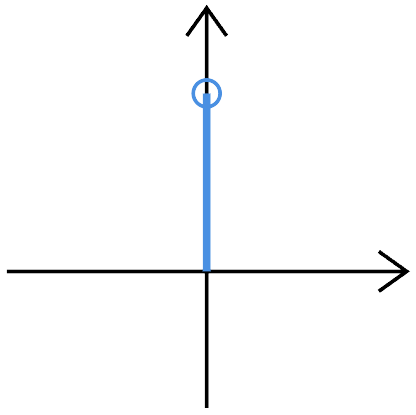
\includegraphics[width=0.15\textwidth]{fig/2.11.png}
        \captionof{figure}{}
        \vspace{0 em}
    \end{wrapfigure}
    则$\mathring{A}=\varnothing,\overline{A}=\left\{(0,y)\in\mb{E}^2\left|0\leq y\leq 1\right.\right\}$.
\end{instance}

\vspace{5 em}
\begin{proposition}
    设$X$是一个拓扑空间，$A,B\subset X$，则
    \begin{enumerate}[(i)]
        \item ${(X-A)}^{\circ} = X-\overline{A}$
        \item $\overline{X-A} = X-\mathring{A}$
        \item $\mathring{A}\cap\mathring{B} = {(A\cap B)}^{\circ}$
        \item $\mathring{A}\cup\mathring{B} \subset {(A\cup B)}^{\circ}$
        \item $\overline{A}\cap\overline{B} \supset \overline{A\cap B}$
        \item $\overline{A}\cup\overline{B} = \overline{A\cup B}$
    \end{enumerate}
\end{proposition}
\begin{proof}
    \begin{enumerate}[(i)]
        \item “$\subset$”\, $\forall\, x\in (X-A)^\circ$，则$\exists\, x$的邻域$U,\st x\in U\subset X-A$，所以$U\cap A=\varnothing$.\par
        根据引理\ref{lem:2.10}，$x\notin\overline{A}$，因此$x\in X-\overline{A}$.\par
        “$\supset$”\, $\overline{A}$是闭集，则$X-\overline{A}$是开集，$A\subset\overline{A}\Rightarrow X-\overline{A}\subset X-A$.\par
        所以$X-\overline{A}\subset (X-A)^\circ$.
        \item 将(i)中的$A$替换为$X-A$即可得到.
        \item “$\subset$”\, $\forall\,x\in\mathring{A}\cap\mathring{B}$. 于是存在$x$的邻域$U_1, U_2$使得$x\in U_1\subset A$且$x\in U_2\subset B$.\par
        因此$x\in (U_1\cap U_2)\subset A\cap B$，其中$U_1\cap U_2$为开集，根据引理\ref{lem:2.10}，$x\in{(A\cap B)}^\circ$.\par
        “$\supset$”\, $\left.\begin{array}{lll}
            A\cap B\subset A \Rightarrow {(A\cap B)}^\circ \subset\mathring{A} \\
            A\cap B\subset B \Rightarrow {(A\cap B)}^\circ \subset\mathring{B}
        \end{array}\right\}\Rightarrow (A\cap B)^\circ\subset \mathring{A}\cap\mathring{B}$
        \item $\left.\begin{array}{lll}
            A\subset A\cup B \Rightarrow \mathring{A}\subset{(A\cup B)^\circ} \\
            B\subset A\cup B \Rightarrow \mathring{B}\subset{(A\cup B)}^\circ
        \end{array}\right\}\Rightarrow (A\cup B)^\circ\subset \mathring{A}\cup\mathring{B}$.\par
        反之不一定成立，例如$[\mb{R}_\mathrm{std},A=(-1,0],B=(0,1)]$，则$\mathring{A}\cup\mathring{B}=(-1,0)\cup(0,1)$，但$(A\cup B)^\circ=(-1,1)$.
    \end{enumerate}
\end{proof}

\begin{definition}{极限点}
    设$X$是一个拓扑空间，$A\subset X$，$x\in X$. 如果$x$的每个邻域都包含$A$中异于$x$的点，则称$x$是$A$的一个\textbf{极限点}(或\textbf{聚点}). $A$的所有极限点的集合记作$A'$.
\end{definition}
上述定义被称为极限点的原因是，如果一个点是极限点，那么我们就可以从每个邻域中选出一个点，这些点列构成了一个收敛的序列.下面给出$x$是$A$的极限点的一个等价描述：
\begin{note}
    $x$是$A$的极限点 $\Leftrightarrow x\in\overline{A-\{x\}}$.
\end{note}
通过这个等价描述，可以看出$A'\subset\overline{A}$.\par

\begin{instance}
    (1)\; 考虑$\mb{E}^1$，和$A=[0,1)\cup\{2\}$，$2\notin A'$. 但$1\in A'$.\par
    (2)\; 考虑$\mb{E}^1$，$A=\mb{Q}$，则$\forall\, x\in\mb{E}^1$，$x\in A'$.
\end{instance}

\begin{proposition}
    $X$是一个拓扑空间，$A\subset X$，则$\overline{A}=A\cup A'$.
\end{proposition}
\begin{proof}
    “$\subset$” $\forall\,x\in\overline{A}$，假设$x\notin A$，则根据引理\ref{lem:2.10}，$x$的任意邻域$U$都与$A$相交.\par
    又因为$x\notin A$，$U\cap A$必须包含除$x$以外的一点，因此$x\in A'$.\par
    “$\supset$” $A\subset\overline{A},A'\subset\overline{A}$.所以$A\cup A'\subset\overline{A}$.
\end{proof}

从这个定理可以得到以下的引理：

\begin{corollary}
    $A\subset X$是闭集$\Leftrightarrow A$包含其所有极限点，即$A'\subset A$.
\end{corollary}
上述引理的正确性是显然的，$A$是闭集$\Leftrightarrow A=\overline{A}=A\cup A'\Leftrightarrow A'\subset A$.\par

\begin{definition}{边界}
    设$X$是一个拓扑空间，$A\subset X$，则$A$的\textbf{边界}是指$\overline{A}-\mathring{A}$，记作$\partial A$.
\end{definition}

\begin{instance}
    在$\mb{E}^2$中，取$A=\{(x,y)\in\mb{E}^2|x^2+y^2\leq 1\}$，则$\partial A=A'-\mathring{A}=\{(x,y)\in\mb{E}^2|x^2+y^2=1\}$.
\end{instance}

\begin{instance}
    在$\mb{R}_{fc}$中，取$A=[0,1)$，则$\overline{A}=\mb{R},\mathring{A}=\varnothing,\partial A=\mb{R}$.
\end{instance}

\begin{lemma}
    设$X$是一个拓扑空间，$A\subset X$，$y\in X$，则$y\in\partial A\Leftrightarrow y$的任意邻域都与$A$和$X-A$相交.
\end{lemma}
\begin{proof}
    “$\Rightarrow$”\, $y\in\partial A=\overline{A}-\mathring{A}$.因此$y\in\overline{A}$，由引理\ref{lem:2.10}可知$y$的任意邻域都与$A$相交.\par
    又因为$y\notin\mathring{A}$，$y\in X-\mathring{A}=\overline{X-A}$，所以$y$的任意邻域都与$X-A$相交. \par
    “$\Leftarrow$”\, 上述证明过程相反即可.
\end{proof}



\begin{proposition}
    设$X,Y$是两个拓扑空间，$A\subset X,B\subset Y$，则
    \begin{enumerate}[(1)]
        \item $(A\times B)^\circ=\mathring{A}\times \mathring{B}\subset X\times Y$.
        \item $\overline{A\times B}=\overline{A}\times \overline{B}\subset X\times Y$
    \end{enumerate}
\end{proposition}
\begin{proof}
    (2)“$\subset$” $\forall\, (x,y)\in\overline{A\times B}$.假设$(x,y)\notin\overline{A}\times\overline{B}$，则要么$x\notin\overline{A}$，要么$y\notin\overline{B}$.\par
    不妨设$x\notin\overline{A}$，则$\exists\, x$的邻域$U,\st U\cap A=\varnothing$.\par
    $U\times Y$是$(x,y)$在$X\times Y$中的邻域，且$(U\times Y)\cap(A\times B)=(U\cap A)\times (Y\cap B)=\varnothing$.\par
    因此$(x,y)\notin \overline{A\times B}$，矛盾! \par
    “$\supset$” $\forall\,(x,y)\in\overline{A}\times\overline{B}$.设$W$是$(x,y)$在$X\times Y$中的邻域. 则存在$x$的邻域$U$和$y$的邻域$V$使得$(x,y)\in U\times V\subset W$.\par
    由$x\in\overline{A}$且$y\in\overline{B}$，可知$U\cap A\neq\varnothing$且$V\cap B\neq\varnothing$. 于是$(U\times V)\cap(A\times B)=(U\cap A)\times(V\cap B)\neq\varnothing$.\par
    因此$W\cap(A\times B)\neq\varnothing$. 这表明$(x,y)\in\overline{A\times B}$.
\end{proof}











